%%%%%%%%%%%%%%%%%%%%%%%%%%%%%%%%%%%%%%%%%%%%%%%%%%%%%%%%%%%%%%%%%%%%%%%%%%%%%%%%
% Template for USENIX papers.
%
% History:
%
% - TEMPLATE for Usenix papers, specifically to meet requirements of
%   USENIX '05. originally a template for producing IEEE-format
%   articles using LaTeX. written by Matthew Ward, CS Department,
%   Worcester Polytechnic Institute. adapted by David Beazley for his
%   excellent SWIG paper in Proceedings, Tcl 96. turned into a
%   smartass generic template by De Clarke, with thanks to both the
%   above pioneers. Use at your own risk. Complaints to /dev/null.
%   Make it two column with no page numbering, default is 10 point.
%
% - Munged by Fred Douglis <douglis@research.att.com> 10/97 to
%   separate the .sty file from the LaTeX source template, so that
%   people can more easily include the .sty file into an existing
%   document. Also changed to more closely follow the style guidelines
%   as represented by the Word sample file.
%
% - Note that since 2010, USENIX does not require endnotes. If you
%   want foot of page notes, don't include the endnotes package in the
%   usepackage command, below.
% - This version uses the latex2e styles, not the very ancient 2.09
%   stuff.
%
% - Updated July 2018: Text block size changed from 6.5" to 7"
%
% - Updated Dec 2018 for ATC'19:
%
%   * Revised text to pass HotCRP's auto-formatting check, with
%     hotcrp.settings.submission_form.body_font_size=10pt, and
%     hotcrp.settings.submission_form.line_height=12pt
%
%   * Switched from \endnote-s to \footnote-s to match Usenix's policy.
%
%   * \section* => \begin{abstract} ... \end{abstract}
%
%   * Make template self-contained in terms of bibtex entires, to allow
%     this file to be compiled. (And changing refs style to 'plain'.)
%
%   * Make template self-contained in terms of figures, to
%     allow this file to be compiled. 
%
%   * Added packages for hyperref, embedding fonts, and improving
%     appearance.
%   
%   * Removed outdated text.
%
%%%%%%%%%%%%%%%%%%%%%%%%%%%%%%%%%%%%%%%%%%%%%%%%%%%%%%%%%%%%%%%%%%%%%%%%%%%%%%%%

\documentclass[letterpaper,twocolumn,10pt]{article}
\usepackage{report_style}

% to be able to draw some self-contained figs
\usepackage{tikz}
\usepackage{amsmath}

% inlined bib file
% \usepackage{filecontents}
\usepackage{datetime}

% math symbols
\usepackage{amssymb}
\usepackage{amsmath}
\usepackage{subfig}
\microtypecontext{spacing=nonfrench}
% graph visualization
\usepackage{pgfplots}
\usetikzlibrary{positioning,calc,arrows}
\usepackage{float}
\usepackage{stackengine}
\usepackage{xcolor}
\definecolor{lightgreen}{HTML}{b2df8a}
\definecolor{lightblue}{HTML}{a6cee3}
\definecolor{darkblue}{HTML}{247bb5}

%-------------------------------------------------------------------------------
\begin{filecontents}{\jobname.bib}
%-------------------------------------------------------------------------------
@inproceedings{frozenqubits,
author = {Ayanzadeh, Ramin and Alavisamani, Narges and Das, Poulami and Qureshi, Moinuddin},
title = {FrozenQubits: Boosting Fidelity of QAOA by Skipping Hotspot Nodes},
year = {2023},
isbn = {9781450399166},
publisher = {Association for Computing Machinery},
address = {New York, NY, USA},
url = {https://doi.org/10.1145/3575693.3575741},
doi = {10.1145/3575693.3575741},
booktitle = {Proceedings of the 28th ACM International Conference on Architectural Support for Programming Languages and Operating Systems, Volume 2},
pages = {311–324},
numpages = {14},
keywords = {NISQ, Quantum Computing, QAOA},
location = {Vancouver, BC, Canada},
series = {ASPLOS 2023}
}
@misc{qaoa,
      title={A Quantum Approximate Optimization Algorithm}, 
      author={Edward Farhi and Jeffrey Goldstone and Sam Gutmann},
      year={2014},
      eprint={1411.4028},
      archivePrefix={arXiv},
      primaryClass={quant-ph}
}
@Article{Ising,
author={Ising, Ernst},
title={Beitrag zur Theorie des Ferromagnetismus},
journal={Zeitschrift f{\"u}r Physik},
year={1925},
month={Feb},
day={01},
volume={31},
number={1},
pages={253-258},
issn={0044-3328},
doi={10.1007/BF02980577},
url={https://doi.org/10.1007/BF02980577}
}
@article{barabasi,
author = {Albert-László Barabási  and Réka Albert },
title = {Emergence of Scaling in Random Networks},
journal = {Science},
volume = {286},
number = {5439},
pages = {509-512},
year = {1999},
doi = {10.1126/science.286.5439.509},
URL = {https://www.science.org/doi/abs/10.1126/science.286.5439.509},
eprint = {https://www.science.org/doi/pdf/10.1126/science.286.5439.509}
}

@misc{panchenko2014introduction,
      title={Introduction to the SK model}, 
      author={Dmitry Panchenko},
      year={2014},
      eprint={1412.0170},
      archivePrefix={arXiv},
      primaryClass={math.PR}
}

@article{Panchenko_2012,
	doi = {10.1007/s10955-012-0586-7},
  
	url = {https://doi.org/10.1007%2Fs10955-012-0586-7},
  
	year = 2012,
	month = {sep},
  
	publisher = {Springer Science and Business Media {LLC}
},
  
	volume = {149},
  
	number = {2},
  
	pages = {362--383},
  
	author = {Dmitry Panchenko},
  
	title = {The Sherrington-Kirkpatrick Model: An Overview},
  
	journal = {Journal of Statistical Physics}
}

@inproceedings{RGCG,
author = {Wilson, David Bruce},
title = {Generating Random Spanning Trees More Quickly than the Cover Time},
year = {1996},
isbn = {0897917855},
publisher = {Association for Computing Machinery},
address = {New York, NY, USA},
url = {https://doi.org/10.1145/237814.237880},
doi = {10.1145/237814.237880},
booktitle = {Proceedings of the Twenty-Eighth Annual ACM Symposium on Theory of Computing},
pages = {296–303},
numpages = {8},
location = {Philadelphia, Pennsylvania, USA},
series = {STOC '96}
}
\end{filecontents}

%-------------------------------------------------------------------------------
\begin{document}
%-------------------------------------------------------------------------------

%don't want date printed
\date{08.06.2023}

% make title bold and 14 pt font (Latex default is non-bold, 16 pt)
\title{\Large \bf FrozenQubits:\\ A report on the methodology and its utility in sparse quantum programs}

\author{
{\rm Baraa Alnassan}\\
Technical University of Munich
\and
{\rm Leo Schultheiß}\\
Technical University of Munich
} % end author

\maketitle

%-------------------------------------------------------------------------------
\begin{abstract}
%-------------------------------------------------------------------------------
FrozenQubits~\cite{frozenqubits} is a technique that boosts the fidelity of Quantum Approximate Optimization Algorithm (QAOA)~\cite{qaoa} by skipping hot-spot nodes. In FrozenQubits, a node with the highest degree of connectivity (hot-spot node) which corresponds to qubits with the highest number of CNOTs is frozen by substituting the value of each qubit with its two possibilities, -1 and +1.\\
This partitions the state-space of the given problem into two smaller problems whose corresponding QAOA circuits are significantly improved. This article is supposed to give an overview of the aforementioned method, as well as analyze its usefulness in more general quantum circuits.
\end{abstract}
%-------------------------------------------------------------------------------
\section{Introduction}
%-------------------------------------------------------------------------------
Near intermediate scale quantum Computers (NISQ Computers) pose an emerging field of research as the qubit count of state-of-the-art systems increases. Currently these qubits are still noisy, so larger quantum programs tend to get high error rates. Thus current development is focused on utilizing the current systems to the greatest extent. In this report we will present one of these methods and introduce the different applications of this method on various quantum circuits.
% and our research building on this method.
%-------------------------------------------------------------------------------
\section{FrozenQubits}
%-------------------------------------------------------------------------------
The method we will focus on in this report is called FrozenQubits~\cite{frozenqubits}. It provides a method to allow for the execution of quantum approximate optimization algorithm (QAOA) programs on NISQ computers and proposes to do so by trading off smaller circuit size for a greater number of circuits to be run.
%-------------------------------------------------------------------------------
\subsection{Background}
%-------------------------------------------------------------------------------
This section will lay the groundwork for the specific optimization problem the original paper had regarded. It is known as \textit{Ising Hamiltonian}, which was first represented as the QAOA~\cite{qaoa} Equation (\ref{Hamiltonian}), where $z_i\in \{-1,+1\}$ and $h_i, J_{ij},\text{offset}\in\mathbb{R}$ are given by the Ising statistical mathematical model of ferromagnetism~\cite{Ising}.
\begin{equation}\label{Hamiltonian}
    H_Z:=C(z)=\sum^{N-1}_{i=0}h_iz_i+\sum^{N-1}_{i=0}\sum^{N-1}_{j=i+1}J_{ij}z_iz_j+\text{offset}
\end{equation}
Then the circuit parameters were tuned to find the optimum value for equation (\ref{Hamiltonian}), which is computationally expensive on classical computers, but QAOA promises speed-up by accelerating this step. FrozenQubits~\cite{frozenqubits} makes use of this acceleration as seen in \ref{results}.
%-------------------------------------------------------------------------------
\subsection{Methodology}\label{methodology}
%-------------------------------------------------------------------------------
In this section we will explain, how FrozenQubits~\cite{frozenqubits} promises to speed up QAOA. The method makes use of the tendency for the degree of nodes in a connectivity graph to follow the power law. Similar to how there are few airports with flights going to most other airports and most airports only having flights to few other airports, most qubits in quantum programs are only connected to few others, and few qubits being connected to a lot of others. FrozenQubits~\cite{frozenqubits} makes use of these highly connected qubits by, as the name suggests, "freezing" them through substitution with $-1$ and $+1$. The $z_i$ are represented by individual qubits, so this results in equation (\ref{Hamiltonian}) being split into two separate equations, with $z_k$ representing the frozen qubit $k$. One with $z_k=+1$ (\ref{Hamiltonian_+1}) and one with $z_k=-1$ (\ref{Hamiltonian_-1}).
\begin{equation}\label{Hamiltonian_+1}
    H_Z^{z_k=+1}=\sum_{\substack{i=0 \\ i \neq k}}^{N-1} h_i^{z_k=+1}z_i+\sum^{N-1}_{\substack{i=0 \\ i \neq k}}\sum^{N-1}_{\substack{j=i+1 \\ j \neq k}}J_{ij}z_iz_j+\text{offset}^{z_k=+1}
\end{equation}
\begin{equation}\label{Hamiltonian_-1}
    H_Z^{z_k=-1}=\sum_{\substack{i=0 \\ i \neq k}}^{N-1} h_i^{z_k=-1}z_i+\sum^{N-1}_{\substack{i=0 \\ i \neq k}}\sum^{N-1}_{\substack{j=i+1 \\ j \neq k}}J_{ij}z_iz_j+\text{offset}^{z_k=-1}
\end{equation}
As one can see, the most influential change to (\ref{Hamiltonian}), is that every term with $z_k$ was eliminated from the summations. Furthermore the $h_i$ had to be adjusted, to account for the effect of $z_k$ on their neighboring qubits. This can be more intuitively understood by looking at figure \ref{fig:graphs}.
\begin{figure}[H]
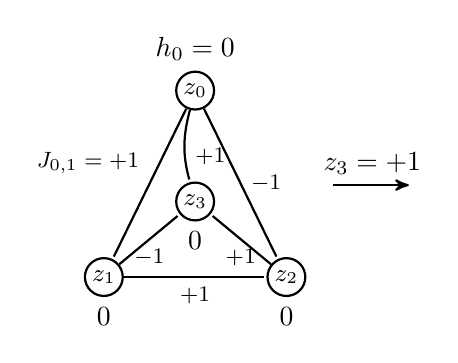
\begin{tikzpicture}[>=stealth',shorten >=1pt,auto,thick,main node/.style={circle,draw,font=\sffamily\small\bfseries,inner sep=0.05cm}]
% nodes
  \node[main node] (0) [label=above:{$h_0=0$}] {$z_0$};
  \node[main node] (3) [label=below:{0}] [below = 0.9cm of 0] {$z_3$};
  \node[main node] (1) [label=below:{0}] [below left = 0.6cm and 0.8cm of 3] {$z_1$};
  \node[main node] (2) [label=below:{0}] [below right = 0.6cm and 0.8cm of 3] {$z_2$};
  %edges
  \path[every node/.style={font=\sffamily\footnotesize}]
    (0) edge node [above left] {$J_{0,1}=+1$} (1)
    (0) edge node [right] {$-1$} (2)
    (0) edge [bend right=15] node [right,pos=0.65] {$+1$} (3)
    (1) edge node [below] {$+1$} (2)
    (1) edge node [below] {$-1$} (3)
    (2) edge node [below] {$+1$} (3);

    \draw[black,->] (1.75cm,-1.2cm) -- (2.75cm,-1.2cm) node[midway,above] {$z_3=+1$};
\end{tikzpicture}
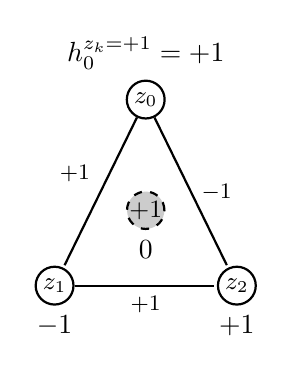
\begin{tikzpicture}[>=stealth',shorten >=1pt,auto,thick,
main node/.style={circle,draw,font=\sffamily\small\bfseries,inner sep=0.05cm},
gray node/.style={circle,draw,dashed,fill={black!20!white},font=\sffamily\small\bfseries,inner sep=0cm}]
% nodes
  \node[main node] (0) [label=above:{$h_0^{z_k=+1}=+1$}] {$z_0$};
  \node[gray node] (3) [label=below:{$0$}] [below = 0.9cm of 0] {$+1$};
  \node[main node] (1) [label=below:{$-1$}] [below left = 0.6cm and 0.8cm of 3] {$z_1$};
  \node[main node] (2) [label=below:{$+1$}] [below right = 0.6cm and 0.8cm of 3] {$z_2$};
  %edges
  \path[every node/.style={font=\sffamily\footnotesize}]
    (0) edge node [above left] {$+1$} (1)
    (0) edge node [right] {$-1$} (2)
    (1) edge node [below] {$+1$} (2);
\end{tikzpicture}
\caption{\label{fig:graphs}"Freezing" of node $z_3$ by substitution with $+1$ and resulting circuit graph with altered topology and $h_i$.}
\end{figure}
Each of these resulting equations, where has been $z_k$ substituted now represent a sub-problem of the original problem (\ref{Hamiltonian}). Overall the number of operations in each of these equation got reduced, but the number of equations doubled. Thus the number of CNOTs and the quantum circuit size got reduced, however now both of these equations are required to be evaluated separately and the results combined. Therefore FrozenQubits~\cite{frozenqubits} creates a trade-off between circuit size and the number of circuits needed to run to solve the entire equation.\\
By applying the method multiple times, thus "freezing" further qubits, the resulting circuit size can be further reduced, however this leads to a doubling of the number of circuits that are generated each time the method is applied. So by freezing $m$ qubits $2^m$ equations are created. The problem graphs for QAOA usually only have very few nodes with a high degree of connectivity, which is why the paper usually chose $m=1$ or $m=2$.
%-------------------------------------------------------------------------------
\subsection{Overhead}\label{overhead}
%-------------------------------------------------------------------------------
Freezing $m$ qubits will result in $2^m$ sub-problem, this in turn will increase the overhead due to several reasons, one of them being that each sub-problem will have to be compiled for execution on a quantum computer, which in turn will add an exponential compilation overhead. Another reason is each sub-problem has to be computed separately and its output has to be concluded with other sub-problems to find the solution to the main problem.
%-------------------------------------------------------------------------------
\subsubsection{Compilation Cost}\label{cost}
By freezing $m$ qubits we generated $2^m$ sub-circuits. However, we only need to compile one circuit, because these circuits only differ in the angles of their rotation gates. This is due to the fact that, the Hamiltonian of each sub-problem only varies in the coefficients and offset values, thus only adjusting the first compiled circuit to fit all other sub-circuits is needed.
%-------------------------------------------------------------------------------
\subsubsection{Trimming Sub-circuits}
As we have seen in section \ref{methodology}, when we freeze a qubit, two sub-circuits will be created as a result by substituting the two possibilities $\{-1, +1\}$ in the Hamiltonian equation (\ref{Hamiltonian}).\\
When all linear coefficients in the equation are set to zero, the sign of $J_{ij}$ depends solely on the value of the multiplication of $z_i$ and $z_j$. By substituting these values we get the following equation:
\begin{equation}
    H_Z := C(z) = \sum^{N-1}_{i=0}\sum^{N-1}_{j=i+1}\smash{{}^+_-}J_{ij}
\end{equation}
From the equation above we can deduce that the state-space of all Hamiltonian with zero linear coefficients are symmetric, so that $C(z) = C(-z)$.
%-------------------------------------------------------------------------------
\subsection{Results}\label{results}
%-------------------------------------------------------------------------------
In this section we will discuss the impact of FrozenQubits~\cite{frozenqubits} on the performance of QAOA and more general power-law graphs. \\
In figure~(\ref{fig:cnots}) the researchers present the results of their method on Barabasi-Albert graphs~\cite{barabasi}, which are randomly generated power-law graphs, in order to determine its effectiveness. As can be seen in sub-figure (\ref{fig:cnots:a}), FrozenQubits successfully reduces the number of CNOTs in the resulting quantum circuit with one qubits being frozen ($m=1)$ compared to the original circuit. This reduction continues with one more frozen qubit ($m=2$). In sub-figure (\ref{fig:cnots:b}) a similar trend was observed, where increasing the number of frozen qubits directly correlates to a lower circuit depth, compared to the original circuit the method was used on.
\begin{figure}[H]
    \centering 
    \subfloat[\label{fig:cnots:a}]{\includegraphics[width=0.49\linewidth]{Results/Results_CNOT.png}}
    \hfill
    \subfloat[\label{fig:cnots:b}]{\includegraphics[width=0.49\linewidth]{Results/Results_CDepth.png}}
    \caption{\label{fig:cnots}Comparison of the impact of FrozenQubits on power-law Barabasi-Albert graphs~\cite{barabasi} on the Number of CNOTs in circuit and the Circuit depth in relation the number of qubits in the circuit}
\end{figure}
Furthermore FrozenQubits~\cite{frozenqubits} showed an increase in compilation time of $10\%$ for $m=1$ compared to the baseline. However, due to the graph construction shortcuts discussed in \ref{overhead}, for $m\geq 3$ compilation time was even reduced, following a decrease in graph size for each frozen qubit. The overall trend can be observed in figure (\ref{fig:compilation}).
\begin{figure}[H]
    \centering
    \includegraphics[width=0.5\linewidth]{Results/Results_Compilation.png}
    \caption{Relative impact on compile time of circuits with FrozenQubits compared to baseline}
    \label{fig:compilation}
\end{figure}
%-------------------------------------------------------------------------------
\section{Research}
%-------------------------------------------------------------------------------
In the following part we will present our own research building on FrozenQubits~\cite{frozenqubits} and how it affects quantum circuits with different topologies than power-law graphs, more specifically \emph{sparse} quantum circuits. Because the method proposed by the paper presents a great opportunity to increase fidelity in power-law graphs it is our goal to generalize this method, to see how useful it might be in more diverse problems. If it would be generally applicable, this would mean that every program could be run at higher fidelity at the cost of more quantum processing. This could be beneficial for many applications requiring a higher degree of resolution in their results not yet reachable/hard to obtain with current systems. We used the number of CNOTs for measuring the impact of FrozenQubits, as they have a large impact on the error rate in circuits and are an easy metric to simulate. An empirical verification of our results in \ref{research:analysis} on real hardware systems is pending.
%-------------------------------------------------------------------------------
\subsection{Sparse circuits}
%-------------------------------------------------------------------------------
For now we will define, what kind of quantum circuits we tested FrozenQubits~\cite{frozenqubits} on. Sparse circuits in this case refers to quantum circuits, in which each qubit is only connected to few other nodes. Because the method presented in the paper was mainly tested on power-law graphs like Barabasi-Albert graphs~\cite{barabasi} this is meant to determine the limit of the benefit in fidelity promised by FrozenQubits~\cite{frozenqubits}.\\
Similar to the original work, we will generalize potential real-world problem graphs using three main types of topologies. 
Examples for the different types of graphs we tested the algorithm on can be seen in figure (\ref{fig:graph_types}) below. Firstly in (\ref{fig:graph_types_regular}) we also tested $2$-regular graphs, as the original paper only covered $3$-regular graphs. And finally an example for randomly generated connected graph (RGCG$_e$)~\cite{RGCG} as in (\ref{fig:graph_types_random}), which are generated with a given edge count $e$. 
\begin{figure}[H]
    \centering
\subfloat[\label{fig:graph_types_regular}]{
    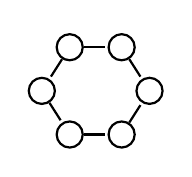
\begin{tikzpicture}[>=stealth',shorten >=1pt,auto,thick,main node/.style=
    {circle,draw,font=\sffamily\small\bfseries}]
    % nodes
      \node[main node] (0) [] {};
      \node[main node] (1) [right = 0.3cm of 0] {};
      \node[main node] (2) [below left = 0.3cm and 0.1cm of 0] {};
      \node[main node] (3)[below right = 0.3cm and 0.1cm of 1] {};
      \node[main node] (4)[below right = 0.3cm and 0.1cm of 2] {};
      \node[main node] (5)[below left = 0.3cm and 0.1cm of 3] {};
      %edges
      \path[every node/.style={font=\sffamily\footnotesize}]
        (0) edge node  {} (1)
        (0) edge node {} (2)
        (1) edge node {} (3)
        (2) edge node {} (4)
        (4) edge node {} (5)
        (5) edge node {} (3);
    \end{tikzpicture}
}
\hspace{1cm}
\subfloat[\label{fig:graph_types_random}]{
    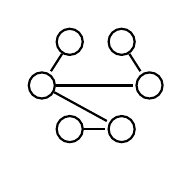
\begin{tikzpicture}[>=stealth',shorten >=1pt,auto,thick,main node/.style=
    {circle,draw,font=\sffamily\small\bfseries}]
    % nodes
      \node[main node] (0) [] {};
      \node[main node] (1) [right = 0.3cm of 0] {};
      \node[main node] (2) [below left = 0.3cm and 0.1cm of 0] {};
      \node[main node] (3)[below right = 0.3cm and 0.1cm of 1] {};
      \node[main node] (4)[below right = 0.3cm and 0.1cm of 2] {};
      \node[main node] (5)[below left = 0.3cm and 0.1cm of 3] {};
      %edges
      \path[every node/.style={font=\sffamily\footnotesize}]
        (0) edge node  {} (2)
        (1) edge node {} (3)
        (2) edge node {} (3)
        (2) edge node {} (5)
        (4) edge node {} (5);
    \end{tikzpicture}
}
    \caption{Sparse graph types the following research is based upon. These include $2$-regular graphs (\ref{fig:graph_types_regular}) and randomly generated connected graphs (\ref{fig:graph_types_random}) (RGCG$_{e=5}$)}
    \label{fig:graph_types}
\end{figure}
%-------------------------------------------------------------------------------
\subsection{Analysis}\label{research:analysis}
%-------------------------------------------------------------------------------
We applied FrozenQubits on different types of graphs that were not mentioned in the paper such as 2-regular graphs and randomly generated connected graphs (RGCG\textsubscript{e})~\cite{RGCG} as shown in figure (\ref{fig:graph_types}). Similar to the previous work in FrozenQubits~\cite{frozenqubits}, in order to be able to study those graphs, we used $J_{i,j}\in \{-1,+1\}$ and $\forall i.h_i=0$ and then applied FrozenQubits on them and studied how the number of CNOTs in the resulting graphs responded. The number of CNOTs in the circuits directly corresponded with the number of edges in each graph, with a factor of $\#CNOTs=2\times \#edges$. The data for the graphs shown in the following sections was generated using the code in this \href{https://github.com/leoschultheiss/FrozenQubitsImplementation}{repository}.
%    - how much would asymmetry of resulting circuits impact the method? (maybe some types of problems will also by symmetric)
%    - disconnected qubits might not be that uncommon (measure?) -> symmetry  restored partially\\
%-------------------------------------------------------------------------------
\subsubsection{2-regular graphs}
%-------------------------------------------------------------------------------
In the following figure (\ref{fig:graph_2rg_rel_cnots}), we show our results for analyzing the impact of FrozenQubits on the number of CNOTs in 2-regular graphs. As is expected and can be seen the number of CNOTs gets reduced for every frozen qubit. However, the impact is very reduced in comparison to power-law type graphs, since every qubit in a 2-regular circuit by definition only has two connections. Therefore the number of connections that can be left out with FrozenQubits stays constant, leading to no further speed up when freezing more nodes. Specifically, when freezing $m$ qubits, the number of CNOTs gets reduced by $2\times 2\times m=4m$.
\begin{figure}[H]
    \centering
    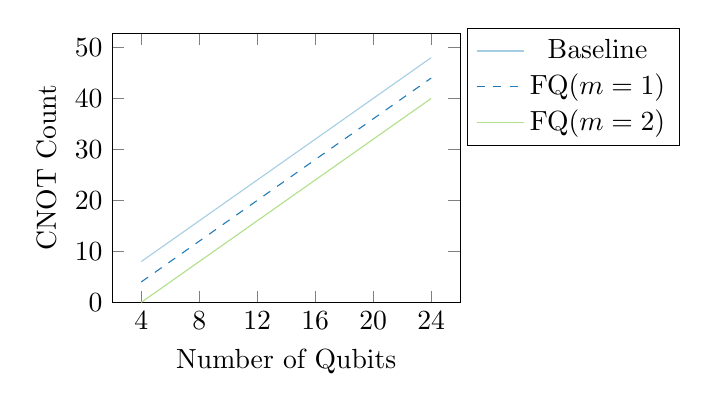
\begin{tikzpicture}
    \begin{axis}[
        xlabel={Number of Qubits},
        ylabel={CNOT Count},
        ymin=0, 
        xtick={4,8,12,16, 20, 24},
        ytick = {0,10,20,30,40,50},
        legend style={at={(1.02,0.58)},
        anchor=south west,legend columns=1},
        width=6cm,
        height=5cm
    ]
    % Load the CSV data
    \pgfplotstableread[col sep=comma]{
        x, y0, y1, y2
        4, 8.0, 4.0, 0.0
        5, 10.0, 6.0, 2.0
        6, 12.0, 8.0, 4.0
        7, 14.0, 10.0, 6.0
        8, 16.0, 12.0, 8.0
        9, 18.0, 14.0, 10.0
        10, 20.0, 16.0, 12.0
        11, 22.0, 18.0, 14.0
        12, 24.0, 20.0, 16.0
        13, 26.0, 22.0, 18.0
        14, 28.0, 24.0, 20.0
        15, 30.0, 26.0, 22.0
        16, 32.0, 28.0, 24.0
        17, 34.0, 30.0, 26.0
        18, 36.0, 32.0, 28.0
        19, 38.0, 34.0, 30.0
        20, 40.0, 36.0, 32.0
        21, 42.0, 38.0, 34.0
        22, 44.0, 40.0, 36.0
        23, 46.0, 42.0, 38.0
        24, 48.0, 44.0, 40.0
    }\datatable
    % Plot the data
    \addplot[lightblue, smooth] table[x=x, y=y0] {\datatable};
    \addplot[darkblue, dashed] table[x=x, y=y1] {\datatable};
    \addplot[lightgreen, smooth] table[x=x, y=y2] {\datatable};
    % Add a legend
    \legend{Baseline, FQ($m=1$), FQ($m=2$)}
    \end{axis}
\end{tikzpicture}
    \caption{Impact of FrozenQubits on the total number of CNOTs in 2-regular graphs for $m\in \{1,2\}$ compared to the original graph}
    \label{fig:graph_2rg_cnots}
\end{figure}
In figure (\ref{fig:graph_2rg_rel_cnots}) we visualize this trend again, where significant changes occur with lower qubit counts. One benefit of using FrozenQubits on 2-regular graphs however, may be the creation of disconnected nodes. For $m\geq 2$ it is possible for one or more nodes to be disconnected from their neighbors, leaving trivial circuits to be computed. These could lead to decreased computational requirements, however as these graphs are highly idealized it is reasonable to assume that this has few applications.
\begin{figure}[H]
    \centering
    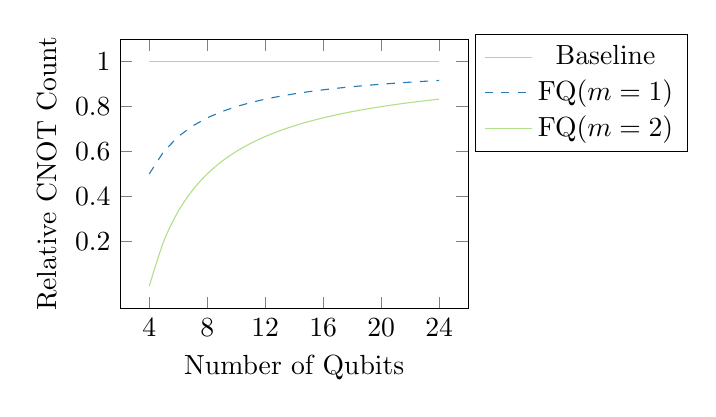
\begin{tikzpicture}
    \begin{axis}[
        xlabel={Number of Qubits},
        ylabel={Relative CNOT Count},
        xtick={4,8,12,16, 20, 24},
        ytick = {0.2,0.4,0.6,0.8,1},
        legend style={at={(1.02,0.58)},
        anchor=south west,legend columns=1},
        % grid=major,
        width=6cm,
        height=5cm
    ]
    % Load the CSV data
    \pgfplotstableread[col sep=comma]{
        x, y0, y1, y2
        4, 1.0, 0.5, 0.0
        5, 1.0, 0.6, 0.2
        6, 1.0, 0.6666666666666666, 0.3333333333333333
        7, 1.0, 0.7142857142857143, 0.42857142857142855
        8, 1.0, 0.75, 0.5
        9, 1.0, 0.7777777777777778, 0.5555555555555556
        10, 1.0, 0.8, 0.6
        11, 1.0, 0.8181818181818182, 0.6363636363636364
        12, 1.0, 0.8333333333333334, 0.6666666666666666
        13, 1.0, 0.8461538461538461, 0.6923076923076923
        14, 1.0, 0.8571428571428571, 0.7142857142857143
        15, 1.0, 0.8666666666666667, 0.7333333333333333
        16, 1.0, 0.875, 0.75
        17, 1.0, 0.8823529411764706, 0.7647058823529411
        18, 1.0, 0.8888888888888888, 0.7777777777777778
        19, 1.0, 0.8947368421052632, 0.7894736842105263
        20, 1.0, 0.9, 0.8
        21, 1.0, 0.9047619047619048, 0.8095238095238095
        22, 1.0, 0.9090909090909091, 0.8181818181818182
        23, 1.0, 0.9130434782608695, 0.8260869565217391
        24, 1.0, 0.9166666666666666, 0.8333333333333334
    }\datatable
    
    % Plot the data
    \addplot[lightblue, smooth] table[x=x, y=y0] {\datatable};
    \addplot[darkblue, dashed] table[x=x, y=y1] {\datatable};
    \addplot[lightgreen, smooth] table[x=x, y=y2] {\datatable};
    
    % Add a legend
    \legend{Baseline, FQ($m=1$), FQ($m=2$)}
    
    \end{axis}
\end{tikzpicture}
    \caption{Relative impact of FrozenQubits on the number of CNOTs in 2-regular graphs}
    \label{fig:graph_2rg_rel_cnots}
\end{figure}
%-------------------------------------------------------------------------------
\subsubsection{Randomly generated connected graphs}
%-------------------------------------------------------------------------------
In randomly generated connected graphs we are more likely to encounter nodes with a higher degree of connectivity compared to the $2$-regular graphs discussed in the last section. Thus, we can expect for FrozenQubits to have a greater impact on the number of CNOTs. This assumption is reaffirmed by figure (\ref{fig:graph_rgcg_cnot}) in that the reduction in the number of CNOTs has almost doubled compared to applying FrozenQubits to $2$-regular graphs. However this is of course still far away from the original results in the paper, when applying the method to Barabasi-Albert graphs.
\begin{figure}[H]
    \centering

    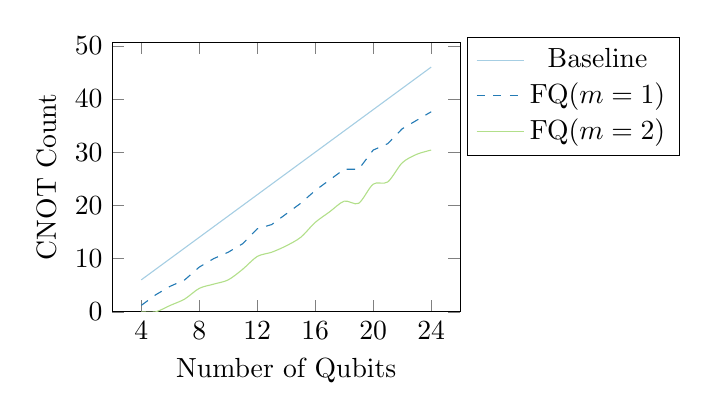
\begin{tikzpicture}
    \begin{axis}[
        xlabel={Number of Qubits},
        ylabel={CNOT Count},
        ymin=0, 
        xtick={4,8,12,16, 20, 24},
        ytick = {0,10,20,30,40,50},
        % grid=major,
        width=6cm,
        height=5cm,
        legend style={at={(1.02,0.58)},
        anchor=south west,legend columns=1},
    ]
    
    % Load the CSV data
    \pgfplotstableread[col sep=comma]{
        x, y0, y1, y2
        4, 6.0, 1.2, 0.0
        5, 8.0, 3.2, 0.0
        6, 10.0, 4.8, 1.2
        7, 12.0, 6.0, 2.4
        8, 14.0, 8.4, 4.4
        9, 16.0, 10.0, 5.2
        10, 18.0, 11.2, 6.0
        11, 20.0, 12.8, 8.0
        12, 22.0, 15.6, 10.4
        13, 24.0, 16.4, 11.2
        14, 26.0, 18.4, 12.4
        15, 28.0, 20.4, 14.0
        16, 30.0, 22.8, 16.8
        17, 32.0, 24.8, 18.8
        18, 34.0, 26.8, 20.8
        19, 36.0, 26.8, 20.4
        20, 38.0, 30.4, 24.0
        21, 40.0, 31.6, 24.4
        22, 42.0, 34.4, 28.0
        23, 44.0, 36.0, 29.6
        24, 46.0, 37.6, 30.4
    }\datatable
    
    % Plot the data
    \addplot[lightblue, smooth] table[x=x, y=y0] {\datatable};
    \addplot[darkblue, dashed] table[x=x, y=y1] {\datatable};
    \addplot[lightgreen, smooth] table[x=x, y=y2] {\datatable};
    
    % Add a legend
    \legend{Baseline, FQ($m=1$), FQ($m=2$)}
    
    \end{axis}
\end{tikzpicture}


    \caption{Impact of FrozenQubits on RGCG$_e$, averaged over 5 generated graphs with $e=\#nodes-1$}
    \label{fig:graph_rgcg_cnot}
\end{figure}    
In the next graph (\ref{fig:graph_rgcg_rel_cnot}) we portray the relative amount of CNOTs in the graph to the original graph with the same data as in (\ref{fig:graph_rgcg_cnot}). The initial benefit of FrozenQubits stems from the fact that by eliminating one node in a graph with fewer nodes this also removes a larger fraction of the existing edges. However this benefit shrinks as qubit count increases, though not quite as extremely as with $2$-regular graphs, because of the nodes with higher degree.
\begin{figure}[H]
    \centering

    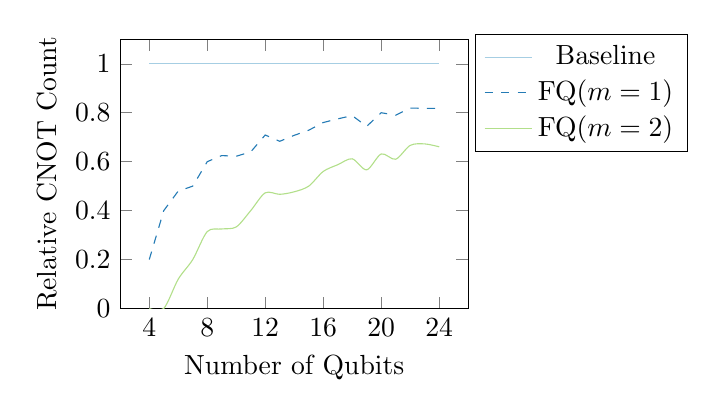
\begin{tikzpicture}
    \begin{axis}[
        xlabel={Number of Qubits},
        ylabel={Relative CNOT Count},
        ymin=0, 
        xtick={4,8,12,16, 20, 24},
        ytick = {0,0.2, 0.4, 0.6, 0.8, 1},
        % grid=major,
        width=6cm,
        height=5cm,
        legend style={at={(1.02,0.58)},
        anchor=south west,legend columns=1},
    ]
    
    % Load the CSV data
    \pgfplotstableread[col sep=comma]{
        x, y0, y1, y2
        4, 1.0, 0.19999999999999998, 0.0
        5, 1.0, 0.4, 0.0
        6, 1.0, 0.48, 0.12
        7, 1.0, 0.5, 0.19999999999999998
        8, 1.0, 0.6, 0.31428571428571433
        9, 1.0, 0.625, 0.325
        10, 1.0, 0.6222222222222222, 0.3333333333333333
        11, 1.0, 0.64, 0.4
        12, 1.0, 0.7090909090909091, 0.4727272727272727
        13, 1.0, 0.6833333333333332, 0.4666666666666666
        14, 1.0, 0.7076923076923076, 0.47692307692307695
        15, 1.0, 0.7285714285714285, 0.5
        16, 1.0, 0.76, 0.56
        17, 1.0, 0.775, 0.5875
        18, 1.0, 0.788235294117647, 0.611764705882353
        19, 1.0, 0.7444444444444445, 0.5666666666666667
        20, 1.0, 0.7999999999999999, 0.631578947368421
        21, 1.0, 0.79, 0.61
        22, 1.0, 0.819047619047619, 0.6666666666666666
        23, 1.0, 0.8181818181818182, 0.6727272727272727
        24, 1.0, 0.8173913043478261, 0.6608695652173913
    }\datatable
    
    % Plot the data
    \addplot[lightblue, smooth] table[x=x, y=y0] {\datatable};
    \addplot[darkblue, dashed] table[x=x, y=y1] {\datatable};
    \addplot[lightgreen, smooth] table[x=x, y=y2] {\datatable};
    
    % Add a legend
    \legend{Baseline, FQ($m=1$), FQ($m=2$)}
    
    \end{axis}
\end{tikzpicture}


    \caption{Relative impact of FrozenQubits on CNOT count in RGCG$_e$, averaged over 5 generated graphs with $e=\#nodes - 1$}
    \label{fig:graph_rgcg_rel_cnot}
\end{figure}  
So overall FrozenQubits can still lead to an improvement in fidelity in less densely connected graphs. However the benefits are a lot less when compared to dense graphs, and importantly they fall off for circuits with more qubits. Therefore FrozenQubits would prove impractical for most sparse circuits.
%-------------------------------------------------------------------------------
\section{Conclusion}
%-------------------------------------------------------------------------------
FrozenQubits was introduced as an application-level software framework to improve the fidelity of Quantum Approximation Optimization Algorithm (QAOA), it works by freezing a qubit or more by substituting the two possibilities in the problem, which partitions the state-space of the problem into smaller sub-spaces. multiple strategies were developed to subside the problem of running the newly created sub-problems individually, such as using the symmetry of the created sub-circuits. In this paper we discussed the impact of FrozenQubits on sparser circuits with lower average connectivity degrees than the ones discussed in the original paper. We discussed the impact of FrozenQubits on sparser circuits on the number of CNOTs. Overall the method produces significantly worse results than with power-law type graphs leading to minor improvements in fidelity at the cost of computational overhead. 
%-------------------------------------------------------------------------------
\bibliographystyle{plain}
\bibliography{\jobname}

%%%%%%%%%%%%%%%%%%%%%%%%%%%%%%%%%%%%%%%%%%%%%%%%%%%%%%%%%%%%%%%%%%%%%%%%%%%%%%%%
\end{document}
%%%%%%%%%%%%%%%%%%%%%%%%%%%%%%%%%%%%%%%%%%%%%%%%%%%%%%%%%%%%%%%%%%%%%%%%%%%%%%%%

%%  LocalWords: FrozenQubits CNOTs QAOA 
